\documentclass[final]{beamer}
\usepackage{etex}

\usetheme{RJH}
\usepackage[utf8]{inputenc}
\usepackage[frenchb]{babel}
\usepackage[orientation=landscape,size=a2,scale=1.2]{beamerposter}
\usepackage[absolute,overlay]{textpos}
\usepackage{url}
\usepackage{auto-pst-pdf}
\usepackage{pst-plot}
\usepackage{graphicx}
\usepackage{color}
\usepackage{hyperref}
\usepackage{amsmath}
\usepackage{amssymb}
\usepackage{pifont}
\newcommand{\cmark}{\ding{51}}%
\newcommand{\xmark}{\ding{55}}%
\usepackage[labelformat=empty]{caption}
\usepackage{framed}
\usepackage{wrapfig}
\usepackage{tikz}
 \usetikzlibrary{arrows}


\setlength{\TPHorizModule}{\paperwidth}
\setlength{\TPVertModule}{\paperheight}

\newcommand{\qedwhite}{\hfill \ensuremath{\Box}}
\newcommand\sbullet[1][.5]{\mathbin{\vcenter{\hbox{\scalebox{#1}{$\bullet$}}}}}

\definecolor{lightgreen}{rgb}{0.0,0.8,0.0}
\definecolor{lightblue}{rgb}{0.3,0.8,1.0}
\definecolor{lightred}{rgb}{0.874,0.180,0.105}
\definecolor{gray}{rgb}{0.4,0.4,0.4}
\definecolor{lightgray}{rgb}{0.8,0.8,0.8}
\definecolor{shadecolor}{rgb}{0.9,0.9,0.9}

\title{Learning to Pivot with Adversarial Networks}
\author{Gilles Louppe, Michael Kagan and Kyle Cranmer\\[1.5ex]
{\tiny
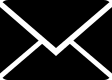
\includegraphics[scale=0.16]{images/mail.png}~\url{g.louppe@ulg.ac.be},~\url{makagan@slac.stanford.edu},~\url{kyle.cranmer@nyu.edu} \\[1.5ex]

\includegraphics[scale=0.18]{images/github.png}~\url{https://github.com/glouppe/paper-learning-to-pivot/}
}}

\footer{}
\date{}

\makeatletter
\newcommand{\superimpose}[2]{%
  {\ooalign{$#1\@firstoftwo#2$\cr\hfil$#1\@secondoftwo#2$\hfil\cr}}}
\makeatother

\begin{document}
\begin{frame}{}


%% Column 1 ==================================================================

\begin{textblock}{0.32}(0.01,0.14)

%% Abstract ------------------------------------------------------------------

\begin{block}{Abstract \phantom{p}}
We address the problem of building a classifier that is robust to changes in the data distribution over a continuous family of data generating processes.  Such domain adaptation problems arise in the scientific context when systematic uncertainties define a set of plausible data generating processes, in cases of fairness with respect to continuous attributes, or generally when one desires a classifier to be invariant to changes in a given feature. Robust inference is achieved through building a pivot, a quantity whose distribution does not depend on the unknown values of the nuisance parameter that parameterize the family of data generating processes.  We introduce and derive theoretical results for a training procedure based on adversarial networks for enforcing the pivotal property on a predictive model.
\end{block}

\vspace{0.5cm}
\begin{block}{Problem Statement \phantom{p}}

\begin{columns}[t]
\begin{column}{0.02\textwidth}
\end{column}
\begin{column}{0.48\textwidth}
Data generating process $p(X, Y, Z)$ \\
$x \in \mathcal{X}$ are the data \\
$y \in \mathcal{Y}$ are the target labels \\
$z \in \mathcal{Z}$ are the nuisance parameters \\
\hspace{1.2cm} continuous or categorical
\end{column}
%\begin{column}{0.02\textwidth}
%\end{column}
\begin{column}{0.48\textwidth}
\textbf{Goal}: Learn regression function $f : \mathcal{X} \to {\cal S}$ with $\smash{s \in {\cal S} = \mathbb{R}^{|{\cal Y}|}}$ 
with parameters $\theta_{f}$ that minimize loss ${\cal L}_f(\theta_f)$ (e.g., the cross-entropy) such that\\
\vspace{0.2cm}
$p(f(X ; \theta_f) = s | z ) = p(f(X ; \theta_f) = s | z^\prime )$
\end{column}
\begin{column}{0.02\textwidth}
\end{column}
\end{columns}

\end{block}

\vspace{0.5cm}
\begin{block}{Method \phantom{p}}



$r := p_{\theta_r}(z | f(X;\theta_f)=s)$ is the adversary model with parameters $\theta_r$ and loss ${\cal L}_r(\theta_f, \theta_r)$. \\
As with generative adversarial networks, $f$ and $r$ are trained simultaneously, which is carried out by considering
the value function
\begin{align}
\nonumber E(\theta_f, \theta_r) = {\cal L}_f(\theta_f) - {\cal L}_r(\theta_f, \theta_r)  &&\text{\hspace{2.35cm} (1)}
\end{align}

that we optimize by finding the minimax solution 
\begin{align}
\nonumber \smash{\hat\theta_f, \hat\theta_r} = \arg \min_{\theta_f} \max_{\theta_r} E(\theta_f, \theta_r)&&\text{\hspace{2.75cm} (2)}
\end{align}

${\cal L}_f$ and ${\cal L}_r$  are respectively set to the
expected value of the
negative log-likelihood of $Y|X$ under $f$ and of $Z|f(X;\theta_f)$ under
$r$: 
\begin{align}
    \nonumber {\cal L}_f(\theta_f) &= \mathbb{E}_{x \sim X}  \mathbb{E}_{y \sim Y|x} [ -\log p_{\theta_f} (y|x) ] &\text{(3)}\\
    \nonumber {\cal L}_r(\theta_f, \theta_r) &= \mathbb{E}_{s \sim f(X;\theta_f)}  \mathbb{E}_{z \sim Z|s} [-\log p_{\theta_r} (z|s)]&\text{(4)}
\end{align}


\vspace{0.2cm}
\begin{center}
\tikzstyle{every node}=[font=\fontsize{10}{11.2}]
\begin{figure}
  
   \def\layersep{1cm}

   \begin{tikzpicture}[shorten >= 1pt, ->, node distance=\layersep,scale=.8]
   \tikzstyle{neuron} = [circle, minimum size=0.25cm, draw=black!20, line width=0.3mm, fill=white]

   % Classifier f
   \node at (2,0) {Classifier $f$};
   \draw (-1,-0.5) rectangle (4,-5.5);

   \path[->, shorten >= 0pt] (-2,-3) edge (-1,-3);
   \node[left] at (-2,-3) {$X$};

   \path[-o, shorten >= 0pt] (1.5,-6.5) edge (1.5,-5.5);
   \node[below] at (1.5,-6.5) {$\theta_f$};

   \path[->, shorten >= 0pt] (3.5,-3) edge (6.5,-3);
   \node[above] at (5.25,-3) {$f(X;\theta_f)$};

   \path[dashed,-] (5.25,-3) edge (5.25,-6.5);
   \node[below] at (5.25,-6.5) {${\cal L}_f(\theta_f)$};

   \foreach \name / \y in {1,...,3}
       \node[neuron] (f-I-\name) at (-0.5,-1-\y) {};

   \foreach \name / \y in {1,...,5}
       \node[neuron] (f-H1-\name) at (-0.5cm+\layersep,-\y cm) {};
   \foreach \name / \y in {1,...,5}
       \node[neuron] (f-H2-\name) at (-0.5cm+3*\layersep,-\y cm) {};

   \node[neuron] (f-O) at (-0.5cm+4*\layersep,-3cm) {};

   \foreach \source in {1,...,3}
       \foreach \dest in {1,...,5}
           \path[black] (f-I-\source) edge (f-H1-\dest);

   \foreach \source in {1,...,5}
       \path[black] (f-H2-\source) edge (f-O);

   \node[black] at (1.5,-3) {...};

   % Adversary r
   \node at (11.75,0) {Adversary $r$};
   \draw (6.5,-0.5) rectangle (11.5,-5.5);

   \node[above] at (13.25,-2) {$\gamma_1(f(X;\theta_f);\theta_r)$};
   \path[-o, shorten >= 0pt] (11,-2.0) edge (15,-2.0);
   \node[above] at (13.25,-3) {$\gamma_2(f(X;\theta_f);\theta_r)$};
   \path[-o, shorten >= 0pt] (11,-3) edge (15,-3);
   \node[above] at (13.25,-4) {$\dots$};
   \path[-o, shorten >= 0pt] (11,-4) edge (15,-4);

   \path[-o, shorten >= 0pt] (9,-6.5) edge (9,-5.5);
   \node[below] at (9,-6.5) {$\theta_r$};

   \foreach \name / \y in {1,...,1}
       \node[neuron] (r-I-\name) at (7,-2-\y) {};

   \foreach \name / \y in {1,...,5}
       \node[neuron] (r-H1-\name) at (7cm+\layersep,-\y cm) {};
   \foreach \name / \y in {1,...,5}
       \node[neuron] (r-H2-\name) at (7cm+3*\layersep,-\y cm) {};

   \node[neuron] (r-O1) at (7cm+4*\layersep,-2cm) {};
   \node[neuron] (r-O2) at (7cm+4*\layersep,-3cm) {};
   \node[neuron] (r-O3) at (7cm+4*\layersep,-4cm) {};

   \foreach \source in {1,...,1}
       \foreach \dest in {1,...,5}
           \path[black] (r-I-\source) edge (r-H1-\dest);

   \foreach \source in {1,...,5}
       \path[black] (r-H2-\source) edge (r-O1);
   \foreach \source in {1,...,5}
       \path[black] (r-H2-\source) edge (r-O2);
   \foreach \source in {1,...,5}
       \path[black] (r-H2-\source) edge (r-O3);

   \node[black] at (9,-3) {...};

   \draw (15,-1.5) rectangle (18,-4.5);
   \path[->, shorten >= 0pt] (16.5,-0.5) edge (16.5,-1.5);
   \node[above] at (16.5,-0.5) {$Z$};
   \path[->, shorten >= 0pt] (16.5,-4.5) edge (16.5,-5.5);
   \node[below] at (16.5,-5.5) {$p_{\theta_r}(Z|f(X;\theta_f))$};
   \node at (16.5,-3) {${\cal P}(\gamma_1, \gamma_2, \dots)$};

   \draw[dashed,-] (16.5,-5) -| (12.75,-6.5);
   \node[below] at (12.75,-6.5) {${\cal L}_r(\theta_f, \theta_r)$};

   \end{tikzpicture}
   
%       \caption{\tiny Architecture for the adversarial training of a binary classifier
%    $f$ against a nuisance parameters $Z$. The adversary $r$ models the
%    distribution $p(z|f(X;\theta_f)=s)$ of the nuisance parameters as observed only through the output $f(X;\theta_f)$ of the classifier. By
%    maximizing the antagonistic objective ${\cal L}_r(\theta_f, \theta_r)$, the classifier
%    $f$ forces $p(z|f(X;\theta_f)=s)$ towards the prior $p(z)$, which happens
%    when $f(X;\theta_f)$ is  independent of the nuisance parameter $Z$ and therefore pivotal.}
\end{figure}


%}
\end{center}

\end{block}

\end{textblock}



%% Column 2 ==================================================================

\begin{textblock}{0.32}(0.34,0.14)

\begin{block}{Theoretical results \phantom{p}}
\begin{shaded}
\textbf{Proposition 1.}
\textit{If there exists a minimax solution $(\smash{\hat\theta}_f, \smash{\hat\theta}_r)$
for Eqn.~(2) such that
$E(\hat\theta_f, \hat\theta_r) = H({Y|X}) - H(Z)$, then
$f(\cdot;\smash{\hat\theta}_f)$ is both an optimal classifier and a pivotal
quantity.}
\end{shaded}

Proof. (\textit{sketch})\\
\begin{enumerate}[(i)]
\item For fixed $\theta_f$, adversary $r$ is optimal at $\hat{\hat\theta}_r = \arg \max_{\theta_r} E(\theta_f, \theta_r)  = \arg \min_{\theta_r} {\cal L}_r(\theta_f, \theta_r)$,\\
in which case $p_{\hat{\hat\theta}_r}(z|f(X;\theta_f)=s) = p(z|f(X;\theta_f)=s)$ $\forall z, s$, and\\
${\cal L}_r \to \mathbb{E}_{s \sim f(X;\theta_f)} [ H({Z|f(X;\theta_f)=s}) ]$;

\item Value function $E$ can be restated as a function of $\theta_f$ only: \\
$E'(\theta_f) = {\cal L}_f(\theta_f) -  H({Z|f(X;\theta_f)})$; 

\item Have lower bound $H({Y|X}) - H(Z) \leq {\cal L}_f(\theta_f) - H({Z|f(X;\theta_f)})$ \\
where the equality holds at $\smash{\hat\theta}_f = \arg \min_{\theta_f} E'(\theta_f)$ when: \\
 $\sbullet$ $\smash{\hat\theta}_f$ minimizes the negative log-likelihood of $Y|X$ under $f$,
    which happens when $\smash{\hat\theta}_f$ are the parameters
    of an optimal classifier. Then, ${\cal L}_f$ reduces to 
    minimum value $H({Y|X})$. \\
  $\sbullet$ $\smash{\hat\theta}_f$ maximizes the conditional entropy
    $H({Z|f(X;\theta_f)})$, since $H(Z|f(X;\theta)) \leq H(Z)$.
\end{enumerate}


$\Rightarrow$ By assumption, the lower bound is active, thus we have $H(Z|f(X;\theta_f)) = H(Z)$
because of the second condition, which happens exactly when $Z$ and $f(X;\theta_f)$
are independent variables. In other words,  the
optimal classifier $f(\cdot;\smash{\hat\theta}_f)$ is also a pivotal
quantity. \qedwhite

\vspace{0.3cm}

\end{block}

\begin{block}{Illustration \phantom{p}}

\end{block}

\end{textblock}


%% Column 3 ==================================================================

\begin{textblock}{0.32}(0.67,0.14)

\begin{block}{Physics Example \phantom{p}}

\end{block}

\vspace{0.5cm}
\begin{block}{Conclusions \phantom{p}}

{\color{green} \cmark} First step towards understanding variable importances, as computed with a forest of totally randomized trees.

{\color{green} \cmark} Variable importances offer a three-level decomposition of the information provided by the inputs about the output.

{\color{green} \cmark} MDI importances exhibit desirable properties for assessing the relevance of a variable:
\begin{itemize}
\item[-] it accounts for all interaction terms, in a fair and exhaustive way;
\item[-] it is null if and only if the variable is irrelevant;
\item[-] it depends only on the relevant variables;
\end{itemize}

{\color{blue} $\Box$} Fully formalize variable importances of actual Random Forests and variants.

{\color{blue} $\Box$} Characterize the distribution of variable importances in a finite setting.


\end{block}

\end{textblock}




\end{frame}
\end{document}
